% Created 2022-08-09 Tue 17:25
% Intended LaTeX compiler: pdflatex
\documentclass[11pt]{article}
\usepackage[utf8]{inputenc}
\usepackage[T1]{fontenc}
\usepackage{graphicx}
\usepackage{longtable}
\usepackage{wrapfig}
\usepackage{rotating}
\usepackage[normalem]{ulem}
\usepackage{amsmath}
\usepackage{amssymb}
\usepackage{capt-of}
\usepackage{hyperref}
\date{\today}
\title{}
\hypersetup{
 pdfauthor={},
 pdftitle={},
 pdfkeywords={},
 pdfsubject={},
 pdfcreator={Emacs 28.1 (Org mode 9.5.2)}, 
 pdflang={English}}
\makeatletter
\newcommand{\citeprocitem}[2]{\hyper@linkstart{cite}{citeproc_bib_item_#1}#2\hyper@linkend}
\makeatother

\usepackage[notquote]{hanging}
\begin{document}

\tableofcontents


\section{Demographic Trends in Treatment Response to Pain Reprocessing Therapy for Chronic Lower Back Pain}
\label{sec:org5437eb3}
(Note: if you are reading the PDF of this file from the git
repository, it may be out of date. It is included in the repo for
convenience but the canonical writeup is in the org file in the repo).
\subsection{Introduction}
\label{sec:org3356f4c}

Chronic lower back pain (cLBP) is the leading cause of disability
world wide and, because of an aging population, the problem is getting
worse (\citeprocitem{4}{Hartvigsen et al., 2018}). Treatment practices in the United
States in particular have indicated a link between cLBP and the opiod
epidemic (\citeprocitem{7}{Shipton et al., 2018}). Ashar et al investigates the
effectiveness of pain reprocessing therapy (PRT) on cLBP and finds a
non-trivial effect (\citeprocitem{2}{Ashar et al., 2022}). In this writeup I analyze
the demographic data associated with that study and find some
compelling correlations between demographic variables and the
effectiveness of both PRT and the open placebo (Saline).

\subsection{Summary of Ashar et all 2022 Results}
\label{sec:org04b11bc}

Subjects in the Ashar study were placed into one of three groups: Pain
Reprocessing Therapy, saline injection in the lower back, and standard
of care(\citeprocitem{2}{Ashar et al., 2022}). PRT consisted of one telehealth
session and 8 sessions with PRT specialized
therapists(\citeprocitem{2}{Ashar et al., 2022}). The saline injection was an open
placebo(\citeprocitem{2}{Ashar et al., 2022}). Patients were tracked for 12 months
after treatment to determine the long term effectiveness of each
intervention using a variety of standardized questionaires covering
cLBP symptoms and other pertinent information(\citeprocitem{2}{Ashar et al., 2022}).

The results relevant to this analysis are succinctly summarized
by Figure \ref{fig:org91a3f3b}.

\begin{figure}[htbp]
\centering
\includegraphics[width=.9\linewidth]{./figures/bpi_intensity_by_group.png}
\caption{\label{fig:org91a3f3b}PRT is effective at mitigating cLBP (compared to Saline and SOC).}
\end{figure}
The question examined in this analysis is how demographics interacts
with treatment.

\subsection{Demographic Data}
\label{sec:org6be84ae}

Ashar and his colleagues made their data sets available to the public
(\citeprocitem{1}{Ashar et al., 2021}). The included demographic data includes information
about education, ethnicity, hispanic status, employment status,
exercise, handedness, self-reported socioeconomic status, marital
status, age, weight, gender, and backpain length.

These data constitute a mixed space of unordered discrete, ordered
discrete, and ordered continuous variables and thus do not lend
themselves to simple methods of dimensionality
reduction. Nevertheless, it is unlikely that the patient population
fills this abstract space of variability.

\subsection{Dimensionality Reduction of Demographic Data}
\label{sec:org9bbfddb}

To understand whether there are clusters in the demographic data (as a
first step towards understanding the effects of demographic status
alongside the intervention studied here) we trained a variational
auto-encoder(\citeprocitem{5}{Kingma and Welling, 2019}) on this demographic data as a method of
dimensionality reduction. An auto-encoder is a simple neural network
which is charged with reproducing data placed on its input layer at
its output layer. The utility of such an exercise is that the middle
layer of such a network typically consists of a small number of
neurons, which forces the network to encode the input in a small
number of dimensions.

Variational Autoencoders use the inner layer to parameterize a
probability distribution, samples from which are then translated by
the second half of the network into the original output. This exercise
improves the smoothness of the representation of lower dimensional
representation of the data.

In this analysis our variational autoencoder was very simple: it had
one intermediate layer of dimension 3, an inner latent space with
dimension 2, and a symmetric decoder (with the exception of a dropout
layer on the input of the encoder).

After training this network for 30,000 epochs we attained a
two-dimensional representation of the demographic data shown in Figure \ref{fig:org9bfa563}.

\begin{figure}[htbp]
\centering
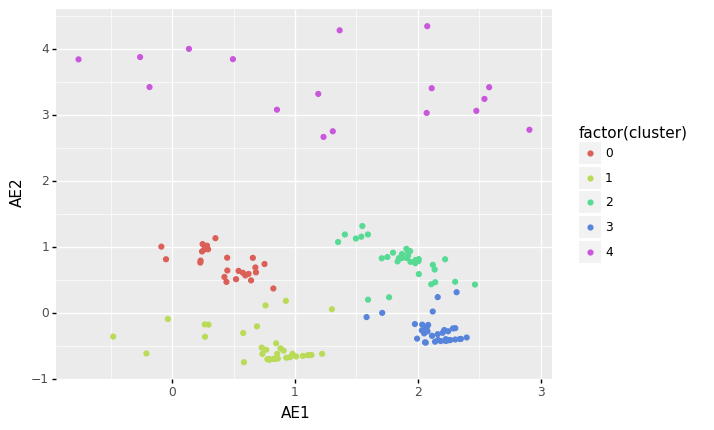
\includegraphics[width=.9\linewidth]{./figures/demo-projection.png}
\caption{\label{fig:org9bfa563}Two dimensional representation of patient demographics generated by a variational autoencoder. A semi-supervised clustering is encoded via point color.}
\end{figure}

A visual inspection of the two-dimensional representation of the data
suggests four clusters and a cloud of outliers. The outlier cloud was
identified by hand and the remaining clusters identified using
spectral clustering(\citeprocitem{6}{Pedregosa et al., 2011}).

\subsection{Automatic Cluster Meaning Identification}
\label{sec:org46fc6a8}

A challenge associated with non-linear dimensionality reduction
combined with cluster analysis is the difficulty of associating
meaning with each cluster since the transformation to the lower
dimensional space is not easily interpreted.

There are several possible solutions to this problem, but here we
employed an unsupervised method: for each cluster, we trained a tree
based model (AdaBoost (\citeprocitem{3}{Freund and Schapire, 1997})) to predict whether a
point would be classified into that cluster. From such a model we can
extract the variables which are most important for the classification
and then calculate summary statistics for each cluster. Using this
method we identified the four distinct clusters as:

\begin{itemize}
\item Younger, Male, Unmarried, White
\item Older, Male, Married, White
\item Lower Weight, Female, Unmarried, White
\item Median Weight, Female, Married, White
\end{itemize}

A pat characterization of the diffuse outlier cloud is not furnished
so easily, but most of these data points are characterized by being
non-white participants.

\subsection{Effect of Cluster Membership on Treatment}
\label{sec:orge4ab3d8}

Now that we have a plausible clustering of the subjects by demographic
character, it is natural to ask whether these demographic identities
correspond to treatment effect differences. This is show in Figure
\ref{fig:org3b2c225}.

\begin{figure}[htbp]
\centering
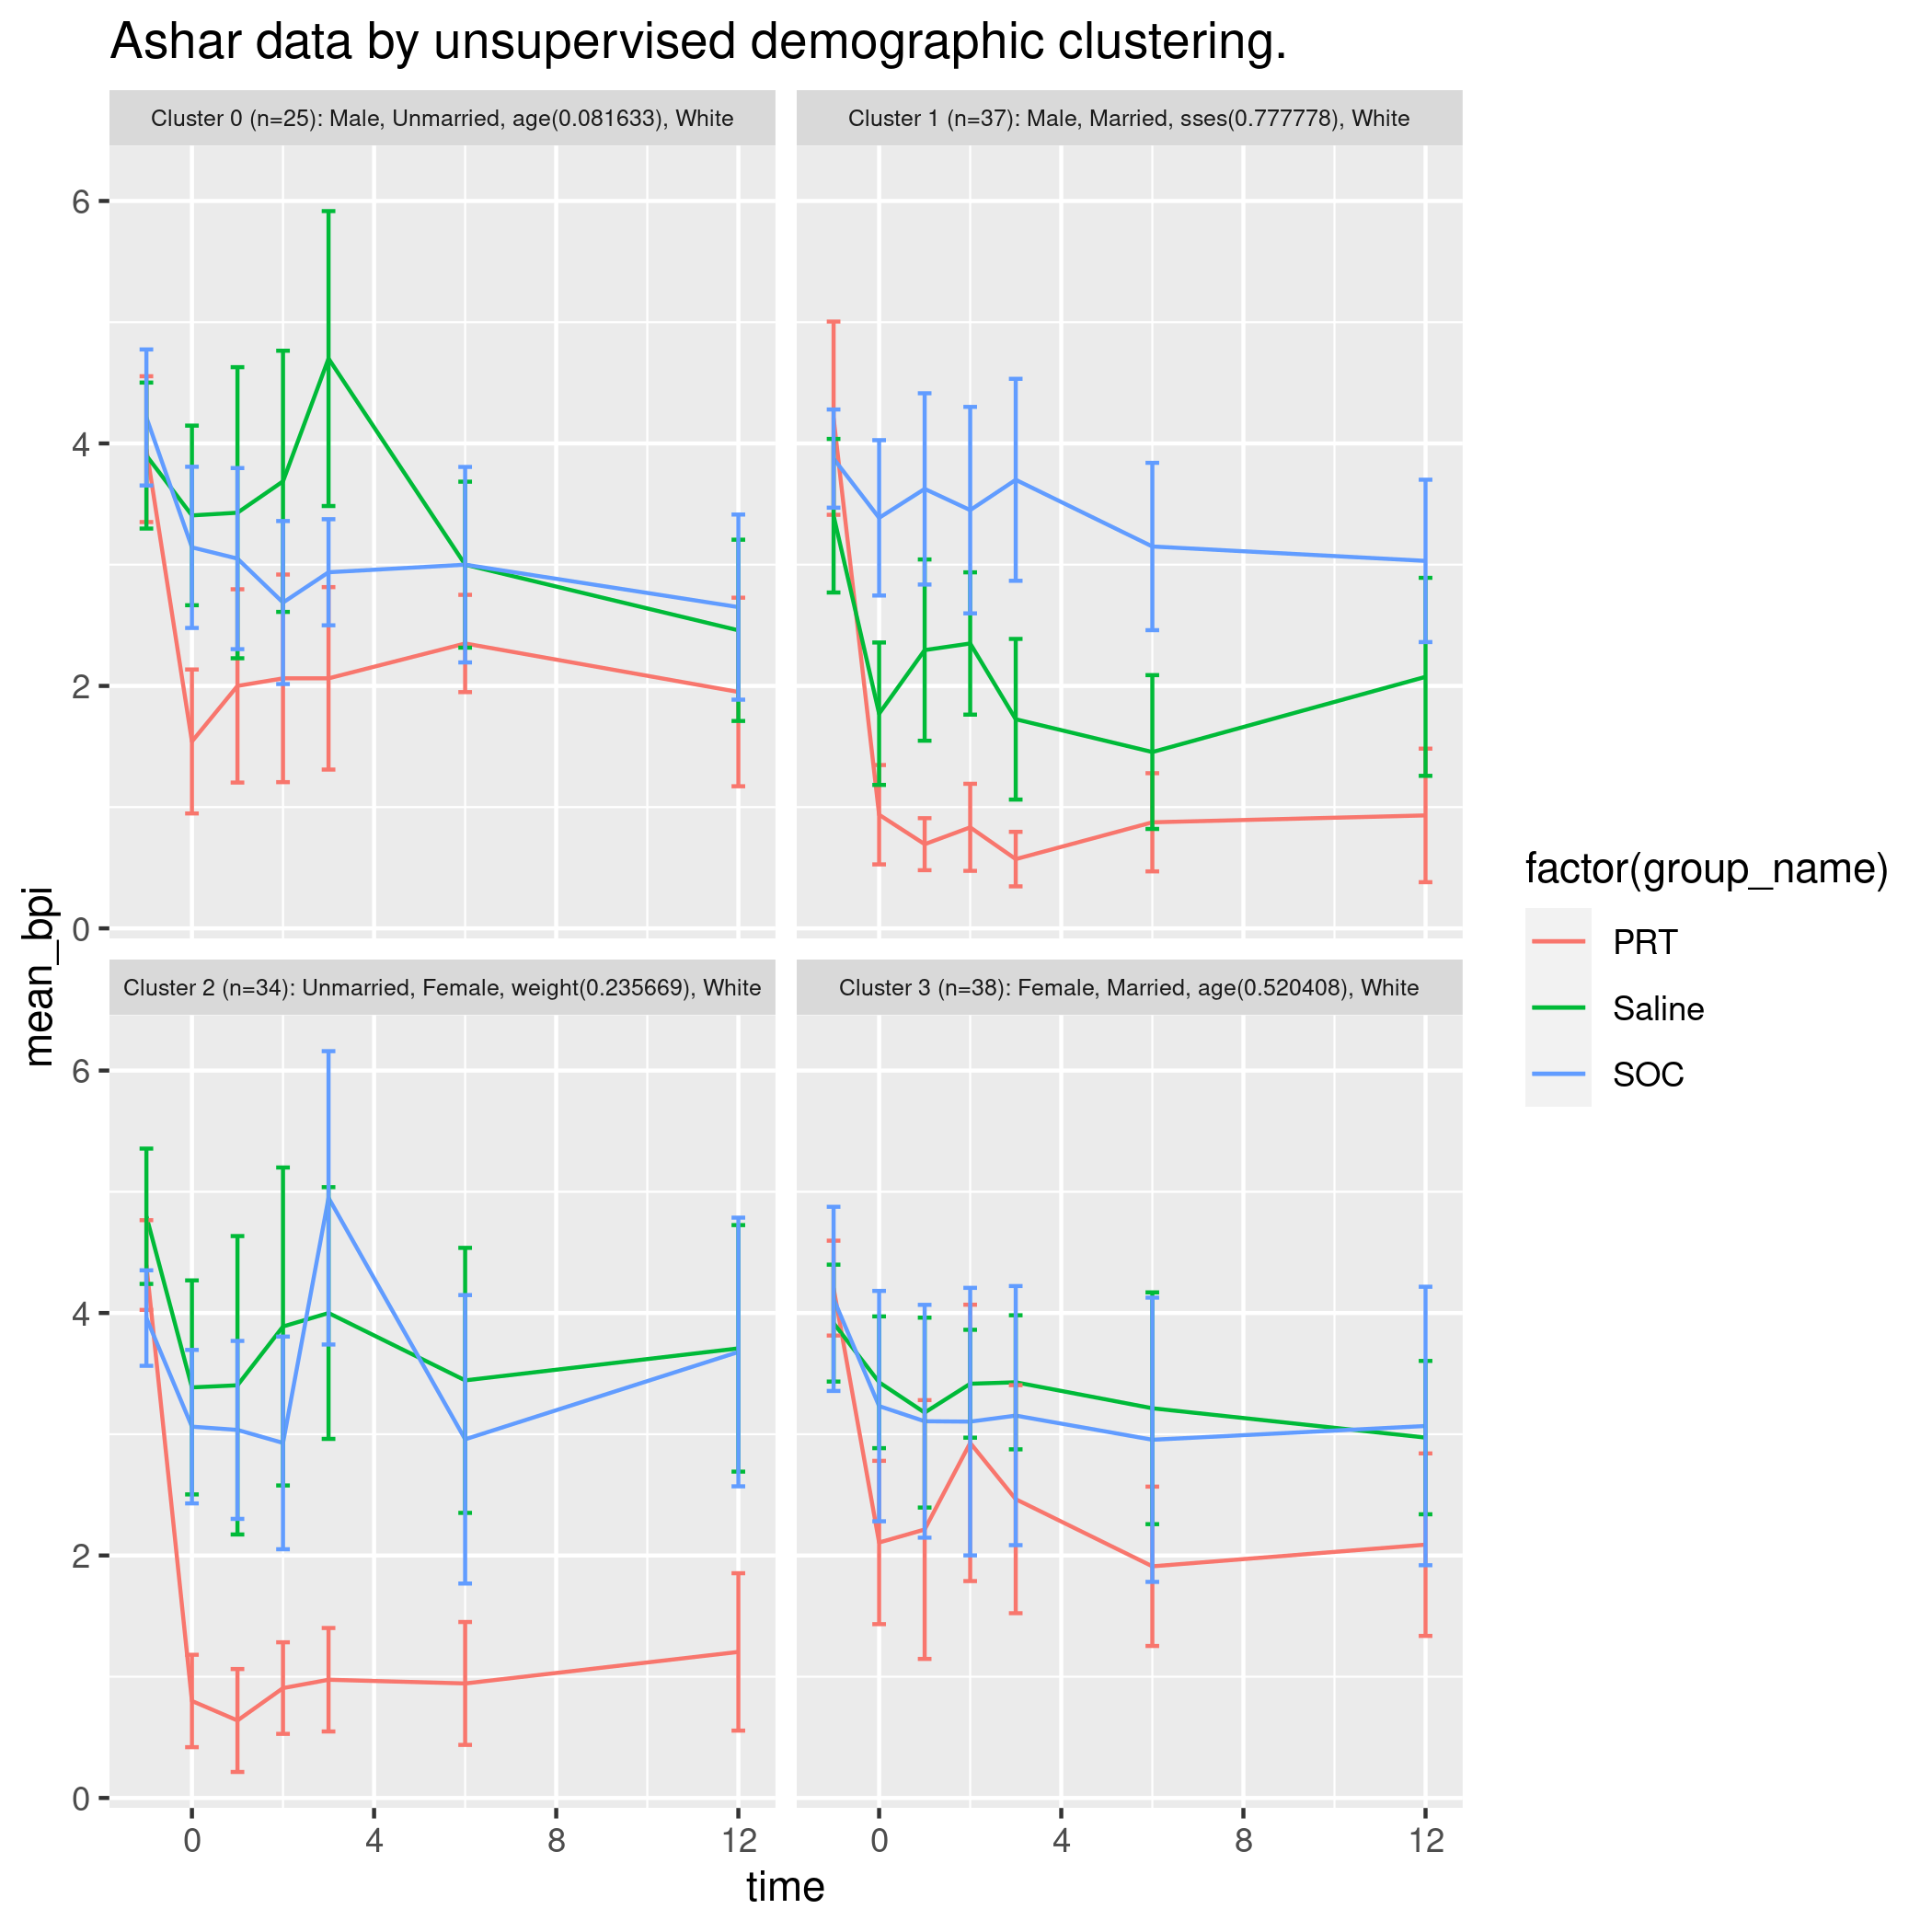
\includegraphics[width=.9\linewidth]{./figures/outcomes_by_demographic_clustering.png}
\caption{\label{fig:org3b2c225}The effect of demographic cluster on the effectiveness of PRT and Saline on cLBP.}
\end{figure}

The picture makes the case that there are strong effects of
demographic group on treatment effect. In particular, older, unmarried
men (who are white, like most participants) and younger, unmarried
women (also white) benefit the most from the treatment. Other
demographic groups benefit less from the intervention.

\section{References}
\label{sec:org3bd7fee}

\hypertarget{citeproc_bib_item_1}{Ashar, Y.K., Gordon, A., Schubiner, H., Uipi, C., Knight, K., Anderson, Z., Carlisle, J., Polisky, L., Geuter, S., Flood, T.F., others (2021). \textit{\href{https://figshare.com/s/1840dc4c0e236a7072ca}{Pain reprocessing therapy for chronic back pain: A randomized controlled trial with functional neuroimaging}}.}

\hypertarget{citeproc_bib_item_2}{Ashar, Y.K., Gordon, A., Schubiner, H., Uipi, C., Knight, K., Anderson, Z., Carlisle, J., Polisky, L., Geuter, S., Flood, T.F., others (2022). Effect of pain reprocessing therapy vs placebo and usual care for patients with chronic back pain: A randomized clinical trial. \textit{Jama Psychiatry} 79, 13–23.}

\hypertarget{citeproc_bib_item_3}{Freund, Y., Schapire, R.E. (1997). A decision-theoretic generalization of on-line learning and an application to boosting. \textit{Journal of Computer and System Sciences} 55, 119–139.}

\hypertarget{citeproc_bib_item_4}{Hartvigsen, J., Hancock, M.J., Kongsted, A., Louw, Q., Ferreira, M.L., Genevay, S., Hoy, D., Karppinen, J., Pransky, G., Sieper, J., Smeets, R.J., Underwood, M., Buchbinder, R., Hartvigsen, J., Cherkin, D., Foster, N.E., Maher, C.G., Underwood, M., van Tulder, M., Anema, J.R., Chou, R., Cohen, S.P., Costa, L.M., Croft, P., Ferreira, M., Ferreira, P.H., Fritz, J.M., Genevay, S., Gross, D.P., Hancock, M.J., Hoy, D., Karppinen, J., Koes, B.W., Kongsted, A., Louw, Q., Öberg, B., Peul, W.C., Pransky, G., Schoene, M., Sieper, J., Smeets, R.J., Turner, J.A., Woolf, A. (2018). \href{https://doi.org/https://doi.org/10.1016/S0140-6736(18)30480-X}{What low back pain is and why we need to pay attention}. \textit{The Lancet} 391, 2356–2367.}

\hypertarget{citeproc_bib_item_5}{Kingma, D.P., Welling, M. (2019). \href{https://doi.org/10.1561/2200000056}{An introduction to variational autoencoders}. \textit{Foundations and Trends® in Machine Learning} 12, 307–392.}

\hypertarget{citeproc_bib_item_6}{Pedregosa, F., Varoquaux, G., Gramfort, A., Michel, V., Thirion, B., Grisel, O., Blondel, M., Prettenhofer, P., Weiss, R., Dubourg, V., Vanderplas, J., Passos, A., Cournapeau, D., Brucher, M., Perrot, M., Duchesnay, E. (2011). Scikit-learn: Machine learning in Python. \textit{Journal of Machine Learning Research} 12, 2825–2830.}

\hypertarget{citeproc_bib_item_7}{Shipton, E.A., Shipton, E.E., Shipton, A.J. (2018). \href{https://doi.org/10.1007/s40122-018-0096-7}{A review of the opioid epidemic: What do we do about it?} \textit{Pain and Therapy} 7, 23–36.}
\end{document}